
\section{Zustandsvariablen-Filter (Biquad-Filter)}

\subsection{Zustandsvariablen-Filter (Biquad-Filter)}
\label{zustandsvariablenfilter}

\begin{minipage}[c]{0.6\columnwidth}
    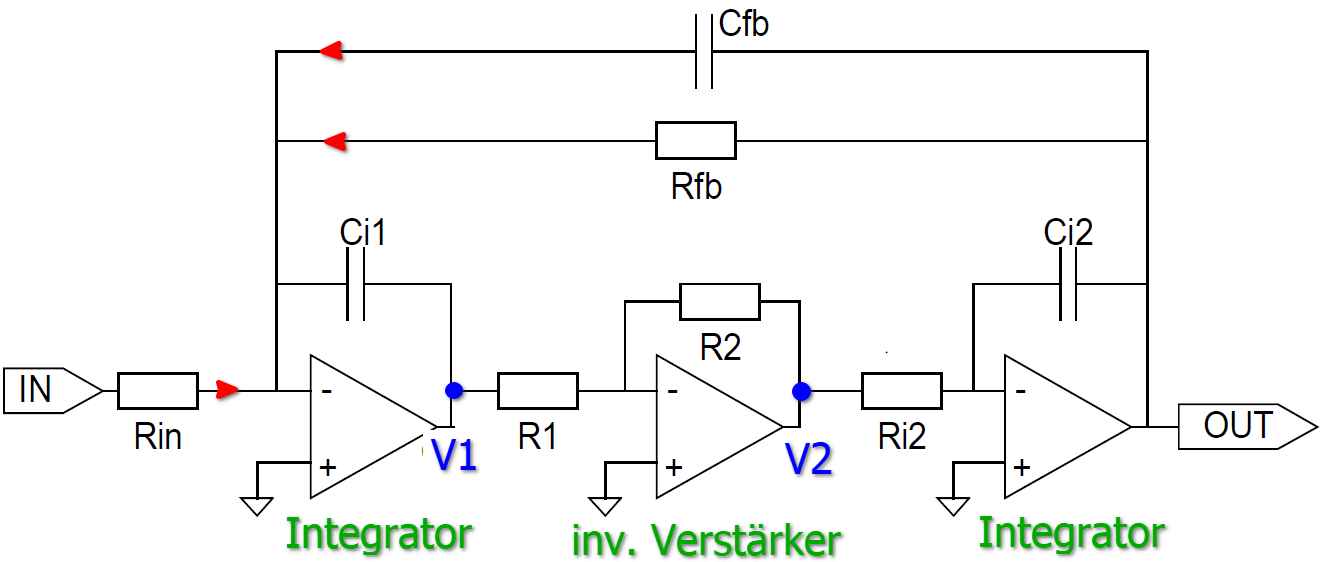
\includegraphics[width=\columnwidth]{images/zustandsvariablenfilter.png}
\end{minipage}
\hfill
\begin{minipage}[c]{0.38\columnwidth}
    \raggedright%
    Mit dieser Topologie sind alle drei \textbf{Parameter} $f_0$, $Q$ und $A_0$ \textbf{frei wählbar!} \\
    An $V_{\rm out}$ herrscht \textbf{Tiefpass-Verhalten.}
\end{minipage}

$$ \boxed{ G(s) = \frac{- \frac{R_{\rm fb}}{R_{\rm in}}}{s^2 \cdot C_{i1} C_{i2} R_{\rm fb} R_{i2} \frac{R_1}{R_2} + s \cdot C_{\rm fb} R_{\rm fb} + 1} } $$

$$ f_0 = \frac{1}{2 \pi \sqrt{C_{i1} C_{i2} R_{\rm fb} R_{i2} \frac{R_1}{R_2}}} \qquad Q = \frac{1}{C_{\rm fb}} \sqrt{C_{i1} C_{i2} \frac{R_1}{R_2 R_{\rm fb}} } 
\qquad A_0 = - \frac{R_{\rm fb}}{R_{\rm in}} $$


\subsubsection{Allgemein: Filter mit mehreren OpAmps}

Mit der Filter-Struktur aus Abschnitt~\ref{zustandsvariablenfilter} können auch Bandpass- und Hochpass-Filter gebildet werden:
\begin{itemize}
    \item \textbf{Tiefpass:} Abgriff beim 3. OpAmp ($V_{\rm out}$ gemäss Abschnitt ~\ref{zustandsvariablenfilter})
    \item \textbf{Bandpass:} Abgriff beim 2. OpAmp (an Knoten V2)
    \item \textbf{Hochpass:} Abgriff beim 2. OpAmp, Einspeisung am neg. Eingang des 2. OpAmps 
\end{itemize}


% CHECK Wohin mit dieser subsection?
% XXX: Allenfalls vor '11.13 Analyse von Filterschaltungen mit Signalflussdiagrammen' verschieben
% CHECK hier?
\subsection{Vorgehen: UTF aus OPV-Filterschaltung ermitteln}
\begin{itemize}
    \item Stromgleichungen (Knotengleichungen) aufstellen
    \item Gleichungen ineinander einsetzen
    \item Umformen nach $G(s) = \frac{V_{\rm out}}{V_{\rm in}}$
\end{itemize}